\section{Related Work}
The literature review is divided into subsequent sections: 1) Position estimation using inertial sensors systems. 2) Sensor fusion in position and orientation estimation.
\subsection{Position estimation using inertial sensor systems}

Inertial sensor systems have been thoroughly researched with the purpose of delivering position estimation of a moving body. Inertial systems are autonomous and independent and do not rely on external information, such as radio signals or electromagnetic waves. Their navigation data have short-term high accuracy, great constancy, and elevated data update rate. They may be applied in an array of distinct positioning methods.
\subsubsection{Pedestrian Dead Reckoning}

Pedestrian dead reckoning (PDR) is among the most explored. PDR combines step detection, step length estimation, and orientation approximations to calculate the absolute position and heading of a walking user. PDR can operate with a single accelerometer, although superior precision and robustness are obtained with more sensors. An Inertial Measurement Unit (IMU) containing several accelerometers, gyroscopes, magnetometers, and even pressure sensors are commonly employed to recognize steps and orientation. Sensors might be body-mounted or shoe-mounted. Pedestrian navigation systems can aid the blind and visually impaired, locating and rescuing firefighters and other emergency workers, hiking, sports, and others. Pedestrian dead reckoning is commonly reviewed in the literature, being subject to studies in various settings.

Ladetto et al. \cite{ladetto2002step} applied PDR in urban and indoor areas seeking to assist blind people reaching unfamiliar locations along with aiming to facilitate emergency coordinators to track rescue workers. The study integrated a GPS receiver with a body-mounted IMU applying pattern recognition to accelerometer signals, determining a user’s step signature.

Stirling et al. \cite{stirling2003innovative} illustrate an experiment exploiting a shoe-mounted sensor prototype that calculates stride length with accelerometers and magnetometers. Their system measures angular acceleration by manipulating pairs of accelerometers as an alternative to gyroscopes.

Several other studies investigate the prospect of using inertial sensor systems to estimate the absolute position and heading of a walking user for multiple purposes \cite{steinhoff2010dead}\cite{weinberg2002using}\cite{kim2004step} \cite{collin2002mems}. The main drawback of PDR is its dependence on step prediction algorithms that must distinguish step direction and step lengths as the user changes pace.

\subsubsection{Strapdown Inertial Integration}
Strapdown inertial integration or strapdown inertial navigation system (SNIS) is another prevalent position method. With SNIS, sensors are usually tightly strapped or attached to the axes of the moving body’s structure, lowering costs and enhancing the system’s reliability. This technique integrates accelerometer and gyroscope measurements to distinguish the variation of position and heading. The strapdown system demands a high-level measurement rate, on average, beyond 2000 Hz. Typically, higher measurement rates translate into more accurate integration readings of position and attitude. Strapdown systems are currently employed in commercial and military applications (airplanes, vessels, ROVs, projectiles) and are a topic of study among scholars.

Jameian et al. \cite{jameian2019robust}  introduced strapdown inertial navigation system to nautical environments, proposing a compensation method against disturbing forces affecting vessel motion caused by rough sea conditions. They aim to resolve attitude determination offset through self-alignment of SNIS by establishing vector observations. The implementation makes use of a quaternion estimator for attitude determination, significantly diminishing computational complexity.

An indoor strapdown inertial navigation with small foot-mounted and self-contained sensor systems was described by Bird et al. \cite{bird2011indoor}. Similar to pedestrian dead reckoning, SNIS also has applications in pedestrian navigation systems, although operating in an utterly distinct fashion. Unlike PDR, the strapdown navigation algorithm traces the entire movement of the foot in between steps. Any movement like walking, running, climbing up or down, moving backward or sideways, sliding, and even jumping can be tracked. This is possible because of a zero-velocity update algorithm (ZVU) which exploits the brief periods of zero velocity when the feet are stationary on the ground.

SNIS and PDR may also be used together, sharing the same inertial sensors. In this case, inertial navigation is incorporated within the multi-sensor integration architecture as the reference system and PDR as an aiding sensor.


With a focus on low-cost inertial motion sensors, Coyte et al. \cite{coyte2013displacement} applied PDR to sporting training and rehabilitation. They propose solutions to acceleration noise accumulation and gyroscope angle error problems. To improve the accuracy of displacement estimation with a low-grade IMU, they developed a zero-velocity update algorithm.

\subsection{Sensor fusion in position and orientation estimation }
Sensor fusion defines the blending of sensory information from two or more sources in a way that generates a more consistent and dependable understanding of the system. One that would otherwise not be possible when these sources were used individually \cite{hall1997introduction}. Fusing multiple inertial systems has raised significant interest and consideration in location and attitude performance improvement. Numerous methods arose in recent times that merge information from various systems such as inertial sensors, GNSS, radar, radio telescopes, signal of opportunity systems like Angle of Arrival (AOA), Time of Arrival (TOA), Received Signal Strength (RSS), and Signal to Noise Ratio (SNR). The combination of multiple sources can help reduce noise with two different sensor types. These separate systems are integrated by fusion filter algorithms which process each input and generate a more precise and reliable output \cite{elmenreich2002introduction}. A substantial sum of distinct solutions designed to assess the orientation of a rigid body regarding a reference frame exist in literature. Two main approaches aimed at sensor fusion exist, Kalman and complementary related filters. A comprehensive analysis of the literature will be conducted seeking to better understand the distinction between algorithms and how do they compare.

\subsubsection{Kalman filter}
The Kalman filter algorithm is a set of mathematical equations that provides a computationally efficient approach to estimate some unknown variables by the detected measurements\cite{welch1995introduction}. Kalman filters operate recursive functions to predict the present state of a linear problem by monitoring the current input data, the previous input data, and the previous state prediction.  Two generally assigned methods for Kalman filter-based sensor fusion are state-vector fusion and measurement fusion. The state-vector fusion method (figure \ref{fig:statekalman}) applies a group of Kalman filters to acquire individual sensor-based state estimates, which are subsequently fused to obtain an enhanced combined state estimate. Measurement fusion (figure \ref{fig:mesearurmentkalman}) approach directly combines the sensor data to achieve a joint measurement and later uses a single Kalman filter to get hold of the final state estimate centered on the fused measurement \cite{mosallaei2007process}.
When applied appropriately, Kalman filters offer highly precise orientation, even with the existence of substantial noise. Nevertheless, Kalman filters are computationally expensive rising hardware cost and latency. They are also of complex implementation, which, shared with computational overhead, can make the algorithm unfeasible for computationally restricted applications. They are regularly useful in a wide-ranging variety of applications and have become a standard method in sensor fusion. Several studies examine the possibility of using Kalman filters to predict a body’s orientation and position by combining multiple sensors. The Kalman filter is founded on recursive Bayesian filtering.
Consequently, the system’s noise is assumed to be Gaussian. Therefore, the Kalman filter is generally suggested for linear systems. For this reason, an extension of the classic Kalman Filter designed for non-linear systems has emerged, recognized as Extended Kalman filter \cite{wilson2019formulation}.


\begin{figure}
   \centering
   \begin{subfigure}[b]{0.45\textwidth}
      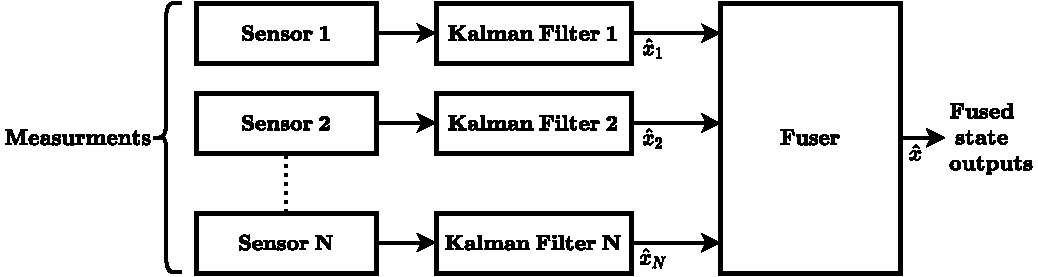
\includegraphics[width=1\linewidth]{figures/kalman1.pdf}
      \caption{}
      \label{fig:statekalman}
   \end{subfigure}
   \begin{subfigure}[b]{0.45\textwidth}
      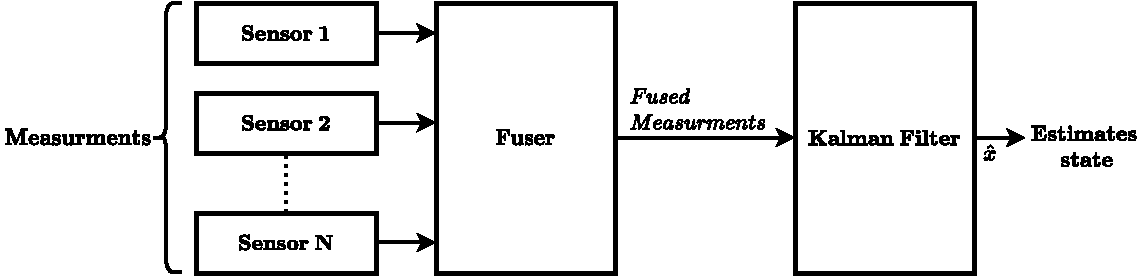
\includegraphics[width=1\linewidth]{figures/kalman2.pdf}
      \caption{}
      \label{fig:mesearurmentkalman}
   \end{subfigure}

   \caption{ Kalman-filter-based multi-sensor data fusion.
      (a) State-vector fusion. (b) Measurement fusion. \cite{mosallaei2007process} }
\end{figure}

Several research works have been conducted on Inertial Navigation Systems and Global Navigation Satellite System integration through data fusion, particularly using the Kalman filter. To overcome the shortcomings linked to the detached functioning of GNSS and INS, Wong et al. \cite{wong1988high} Qi et al. \cite{qi2002direct}, and Nassar et al. \cite{nassar2004improving} combined both systems so that their disadvantages were lessened or eradicated, complementing one another. While GNSS was comparatively more stable and consistent for long periods, INS had a more reliable and comprehensive short-term signal. Updating INS position and velocity with GNSS data corrected error expansion at the same time it delivered more precise estimates. The Kalman Filter attempted to adjust INS information based on the system error model whenever GNSS signals were interrupted or limited. These studies have demonstrated success in satisfying the accuracy requirements of low-precision applications. However, they could not deliver the high-precision positioning some applications required. Hence, other studies attempted to achieve better performance of integrated INS/GNSS systems through the exploration of extended and adaptive Kalman filtering techniques. Mohamed and Schwarz \cite{mohamed1999adaptive} performed an analysis on INS/GNSS alternative integration through an adaptive Kalman filtering technique. Findings reveal that their adaptive Kalman filter outperformed by almost 50\% the conventional filter.

The use of data fusion in autonomous flying units such as Unmanned Aerial Vehicles (UAV) has recently gained particular concern due to the dissemination of consumer-grade quadcopters. In autonomous aerial settings, an accurate altitude reading is crucial to control the position of the flying system. However, such measurements are repeatedly corrupted with signal noise produced by the vehicle’s motors. Hetényi et al. \cite{hetenyi2016sensor} applied a Kalman Filter to fuse the sonar and accelerometer signals, obtaining a considerably improved altitude estimate with minimal error. Similarly, Luo et al. \cite{luo2013uav} combined the UAV sensor system and received signal strength (RSS) in a Kalman filter solution. The study sought to increase position and altitude estimation as well as collision avoidance precision by approximating the distance between the receiver and the transmitter via the use of radiofrequency signals reducing the noise component.

Sharma et al. \cite{sharma2014sensor} present an experiment of Kalman filter-based sensor fusion for extrapolation of a robot’s orientation and depth to obstacle by fusing the inputs from three infrared sensors and an inertial sensor system. The combination of multiple sensor inputs allowed the robot to operate in fault-tolerant applications and enhanced its obstacle avoidance decision making, localization, and orientation estimations.

\subsubsection{Complementary filter}
The complementary filter is considered a simpler approach relatively to the Kalman filter since it is a computationally lightweight solution and straightforward to implement \cite{higgins1975comparison}. This filter takes as input two noisy sensor measurements and assumes one input is mainly formed by high-frequency signals whereas the other is mostly by low-frequency signals. Through a low pass filter, the high-frequency noise of the first input is filtered out. An identical procedure occurs with the second signal, but this time with a high pass filter to remove low-frequency noises, as illustrated in figure \ref{fig:complementary}. Yet, the complementary filter is not especially robust to noisy or biased data since it simply uses currently available information, therefore, has no direct method of compensating for sensor noise \cite{wilson2019formulation}. A conventional application of the complementary filter is to bring together measurements of vertical acceleration and barometric readings to attain an approximation of vertical velocity. Similar to the Kalman filter, new versions built upon the principles of the classic complementary filter have emerged in recent times, such as the Extended Complementary Filter (ECF). They promise a high level of accuracy and enhanced robustness to noise while preserving computational efficiency.

\begin{figure}[!h]
   \centering
   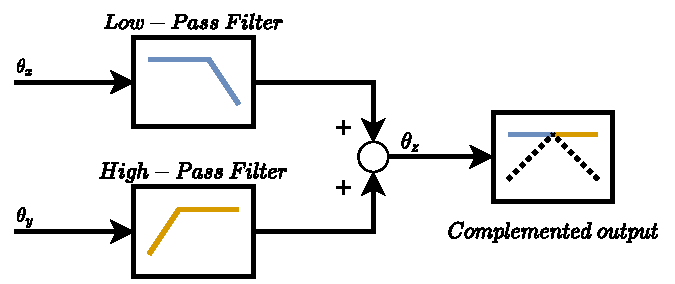
\includegraphics[width=0.7\textwidth]{figures/complementary.pdf}
   \caption{Basic complementary filter \cite{higgins1975comparison} - Two different measurement sources for estimating one variable. The noise properties of the two measurements are such that one source gives good information only in low frequency region while the other is good only in high frequency region. }
   \label{fig:complementary}
\end{figure}

Madgwick et al. \cite{madgwick2020extended} outlined the formulation of an extended complementary filter algorithm and exhibited its applicability as a human motion monitoring wearable. Their design fused magnetic, angular rate, and gravity sensor data to remotely estimate limb orientation in stroke patients performing rehabilitation exercises. They analyzed performance under a range of circumstances and benchmarked alongside other frequently utilized sensor fusion algorithms. They claim an improved computational efficiency of over 30\% when compared with standard alternative algorithms.

A complementary filter designed for sensor fusion in quadrotor UAV employing a low-cost inertial measurement system was proposed by Noordin et al. \cite{noordin2018sensor}. The complementary filter filtered high-frequency signals associated with the gyroscope and low-frequency signals linked to the accelerometer. Findings demonstrate that the complementary filter technique overcame the over drift conundrum related to gyroscopes and was capable of computing attitude angles efficiently.
Euston et al. \cite{euston2008complementary} conducted an analogous study with a non-linear complementary filter for attitude estimation in a UAV utilizing a low-cost IMU. They broadened the experiment to incorporate a model of the longitudinal angle-of-attack corresponding to the UAV’s airframe acceleration using airspeed data. As a result, they could estimate the acceleration of the UAV during continuous turns based on gyroscope and airspeed data. They accomplished attitude filtering performance of similar quality as an extended Kalman filter that fused GPS/INS at a far less computational cost.

\subsubsection{Optimization filters}

Up until recently, there remained mainly two distinct AHRS fusion approaches. One category including the complementary filters, and the other is related to Kalman filtering. Some recent AHRS algorithms have emerged in the literature over the past years. Two of the most prominent are the Mahony and Madgwick algorithms, which have been categorized as optimization filters. Optimization filters obtain orientation by assessing a vector representative of the sensor output at the present orientation and lessening the disparity concerning predicted and observed outputs. Optimization filters are well established for linking accuracy with computational expense and simplicity of implementation \cite{madgwick2020extended}.
Both methods make use of a quaternion representation, which is a four-dimensional complex number representing of an object orientation. Quaternions involve fewer computation time because of their minimal quantity of calculation parameters \cite{ludwig2018comparison}. Additionally, vector rotations are easily executed by quaternion multiplications.
Madgwick et al. \cite{madgwick2010efficient} pioneered a gradient descent fusion algorithm, frequently recognized as ‘Madgwick Algorithm.’ This gradient descent fusion algorithm first obtains a quaternion estimation of the gyroscope output integration and later corrects it with a quaternion from the accelerometer and magnetometer data. Madgwick’s approach guarantees decent attitude estimation at a low computational cost. Further, it tackles the difficulty of the local magnetic disturbances that can influence all the orientation components. By reducing the constraint of the magnetic field vector rotation, it can limit the effect of the magnetic disturbances to only affect the yaw component of the orientation.

\subsubsection{Sensor fusion algorithms comparison}
Some studies have conducted comparison experiments between the sensor fusion algorithms in distinct settings to assess their performance in that unique condition. Ludwig et al. \cite{ludwig2018comparison} compared Madgwick and Mahony in a foot-mounted experiment. Their findings revealed that Madgwick achieved better heading orientation than Mahony when compared to the ground truth. Nonetheless, the performance of Mahony was superior to Madgwick. The same authors tested on \cite{ludwig2018comparisonuav} quadcopters the Extended Kalman Filter, Madgwick, and Mahony filters. Results showed that Mahony delivered a more precise orientation estimation and faster execution time than Madgwick and EKF. Diaz et al. \cite{diaz2015evaluation} present a comparison among Madgwick and Mahony, a basic AHRS estimation algorithm, and the recent algorithm proposed by the authors. The study centered around comparing the performance of Madgwick, Mahony, Extended Kalman Filter, and their own sensor fusion algorithm, emphasizing the behavior under magnetic perturbations. Various examples of movement were analyzed, from carrying the sensor at separate places such as pocket, shoe, and hand. They concluded that their algorithm was slightly less influenced by magnetic perturbations than the others, but overall, the algorithms performed similarly.


% \begin{table}[h!]
%   \begin{center}
%     \caption{Literature categorisation.}
%     \label{tab:table1}
%     \begin{tabular}{l|S|r}
%       \toprule % <-- Toprule here
%       \textbf{Value 1} & \textbf{Value 2} & \textbf{Value 3}\\
%       \midrule % <-- Midrule here
%       1 & 1110.1 & a\\
%       2 & 10.1 & b\\
%       3 & 23.113231 & c\\
%       \bottomrule % <-- Bottomrule here
%     \end{tabular}
%   \end{center}
% \end{table}

\subsection{Thesis Contribution}
With this study, we aim to design and build a low-cost, multipurpose Inertial Navigation System, intending to estimate the orientation and position of a moving object in three-dimensional space. This research additionally proposes introducing an experimental comparison among several established AHRS sensor fusion algorithms such as the Extended Kalman Filter, Madgwick, and Mahony algorithms. Furthermore, a quaternion-based gravity compensation filter will be presented, diminishing the influence of the gravity component on acceleration readings. Our key contribution is to merge IoT with our Inertial System through Long Range (LoRa) communication to perform real-time and long-distance telemetry.